%%=============================================================================
%% Methodologie
%%=============================================================================

\chapter{\IfLanguageName{dutch}{Methodologie}{Methodology}}%
\label{ch:methodologie}

%% TODO: In dit hoofstuk geef je een korte toelichting over hoe je te werk bent
%% gegaan. Verdeel je onderzoek in grote fasen, en licht in elke fase toe wat
%% de doelstelling was, welke deliverables daar uit gekomen zijn, en welke
%% onderzoeksmethoden je daarbij toegepast hebt. Verantwoord waarom je
%% op deze manier te werk gegaan bent.
%% 
%% Voorbeelden van zulke fasen zijn: literatuurstudie, opstellen van een
%% requirements-analyse, opstellen long-list (bij vergelijkende studie),
%% selectie van geschikte tools (bij vergelijkende studie, "short-list"),
%% opzetten testopstelling/PoC, uitvoeren testen en verzamelen
%% van resultaten, analyse van resultaten, ...
%%
%% !!!!! LET OP !!!!!
%%
%% Het is uitdrukkelijk NIET de bedoeling dat je het grootste deel van de corpus
%% van je bachelorproef in dit hoofstuk verwerkt! Dit hoofdstuk is eerder een
%% kort overzicht van je plan van aanpak.
%%
%% Maak voor elke fase (behalve het literatuuronderzoek) een NIEUW HOOFDSTUK aan
%% en geef het een gepaste titel.

Het onderzoek werd uitgevoerd in een iteratieve cyclus, waarbij de verschillende fasen van het project elkaar opvolgden en elkaar beïnvloedden.
Deze sectie beschrijft in grote lijnen de verschillende fasen van het onderzoek, de doelstellingen en de gebruikte methodologieën.

\section{Literatuurstudie}

TODO

\section{Huisgemaakte Data}

Voor het onderzoek en het uitwerken van de PoC software-applicatie, was het belangrijk om zicht te krijgen op de werking van de Eyetracker en de bijhorende software.
Daarom werd deze ontleend uit het Zorglab van HoGent voor een periode van 3 weken. 
Tijdens deze periode werden thuis verschillende opnames gemaakt in een woonkamer met diverse objecten, met de volgende specifieke doelstellingen:
\begin{itemize}
    \item Het leren werken met de Tobii Pro Glasses 3 en de bijhorende software.
    \item Nagaan hoe men de eyetrackingdata kan exporteren naar een bruikbaar formaat via de WiFi-verbinding van de eyetracker.
    \item Een dataset creëren die kan dienen als basis voor het uitwerken van de PoC.
\end{itemize}
Deze opnames werden niet gebruikt voor de uiteindelijke evaluatie van de PoC, aangezien de data afkomstig zijn van tests waarbij de onderzoeker zelf de eyetracker droeg.
Hierdoor is er sprake van mogelijke bias, wat de objectiviteit van de data in het gedrang brengt.

\section{Proof of Concept Software Applicatie}

De kern van dit onderzoek was de ontwikkeling van een Proof-of-Concept (PoC) softwareapplicatie. 
Het hoofddoel van deze fase was het ontwerpen en implementeren van een werkend prototype dat de beoogde workflow ondersteunt: van het importeren van ruwe eyetracking-opnames tot het genereren van geannoteerde data die als basis kan dienen voor analyse. 
De methodologie omvatte de selectie van een passende, moderne technologie-stack (o.a. Python, FastAPI, HTMX, SQLite) gericht op modulariteit en toekomstige uitbreidbaarheid. 
Een significant onderdeel was het ontwerp en de implementatie van een semi-automatische labeling-tool, bedoeld om de efficiëntie van het annotatieproces te verhogen. 
Er werd ingezet op goede software-ontwikkelpraktijken zoals type hinting en containerisatie (Docker) om de onderhoudbaarheid en reproduceerbaarheid te waarborgen. 
De resulterende applicatie, inclusief de architectuur, componenten en technische keuzes, wordt uitvoerig beschreven in Hoofdstuk~\ref{ch:ontwikkeling}.

\section{Experiment in het Zorglab}

Zoals eerder vermeld, werd de thuisopgenomen dataset niet gebruikt voor de evaluatie van de PoC. 
Om een onbevooroordeelde dataset te verkrijgen en om de modaliteiten van de uitwerking te valideren (bijvoorbeeld: invloed van de afstand tussen de Eyetracker en het object, en de aard van de objecten), werd er een gecontroleerd experiment opgezet in het Zorglab van HoGent.
Het doel van dit experiment was om een dataset te creëren die als grond-waarheid diende voor de metrieken die de PoC berekent (bekeken objecten en tijdsduur).
Op de campus werden studenten van diverse opleidingen gevraagd om deel te nemen aan het experiment.
De 14 resulterende opnames werden daarna gelabeld via de labeling-tool van de PoC, met een kwaliteitscontrole om de betrouwbaarheid van de data te waarborgen.
Voor een uitgebreide beschrijving van de opzet en uitvoering van het experiment, inclusief de gebruikte methodologieën, wordt verwezen naar Hoofdstuk~\ref{ch:experiment}.

% \subsection{Opstelling van het Experiment}

% Voorafgaand aan het experiment werden 15 verschillende objecten in de ruimte geplaatst, waarvan elke deelnemer er vijf diende te observeren.
% Er werd gezorgd voor een diverse selectie van objecten, zodat de beperkingen van het systeem konden worden geëvalueerd.
% Ook waren de objecten zo gekozen dat ze relevant waren binnen de context van echte simulaties. De concrete uitwerking hiervan wordt verder toegelicht in de sectie \ref{sec:TODO}.
% De instructies aan de deelnemers waren op een bepaalde plaats in de ruimte te staan, hun blik te richten op de objecten en vervolgens ernaar toe stappen.
% Dit werd voor elk van de vijf objecten herhaald.

% Daarnaast werden er twee afzonderlijke opnames gemaakt door de onderzoeker zelf met als doel het genereren van labelingdata voor het trainen van modellen.
% In deze opnames werd gedurende 30 seconden naar elk object gekeken vanuit verschillende invalshoeken.
% De eerste opname werd gemaakt met de objecten op dezelfde locatie als in het experiment met de deelnemers.
% In de tweede opname werden de objecten op een andere plaats gezet, om te kunnen nagaan of veranderingen in de achtergrond een invloed hebben op de herkenbaarheid of detectie van objecten in de analysefase.
% Deze extra data diende als grondlaag voor het labelen van de objecten en het valideren van de robuustheid van het systeem bij variërende omgevingsfactoren.

% \subsection{Data Labeling}

% De verzamelde data uit het experiment werd gelabeld met behulp van een semi-automatische labeling-tool die ontwikkeld werd binnen de PoC.
% Binnen elke opname werd er op elk object een aantal maal geklikt, waarna de applicatie het object doorheen de video volgde.
% Op deze manier kreeg elk object een segmentatie-masker binnen elke videoframe.
% Daarna werden deze segmentatie-maskers gefilterd op basis van de blikpunten van de deelnemer doorheen de video.

% Op die manier werd een dataset opgebouwd die voor elk frame informatie bevat over welke objecten effectief bekeken werden.
% Aan de hand van deze informatie kon er ook berekend worden hoelang een deelnemer naar elk object gekeken had.

% Ter controle van de labelingkwaliteit werd automatisch een video gegenereerd waarin per frame het segmentatiemasker, de bounding box, het objectlabel en het blikpunt visueel weergegeven werden.
% Deze video werd manueel nagekeken om mogelijke labelingfouten op te sporen en de betrouwbaarheid van de dataset te waarborgen.

% \begin{figure}[H]
%   \centering
%   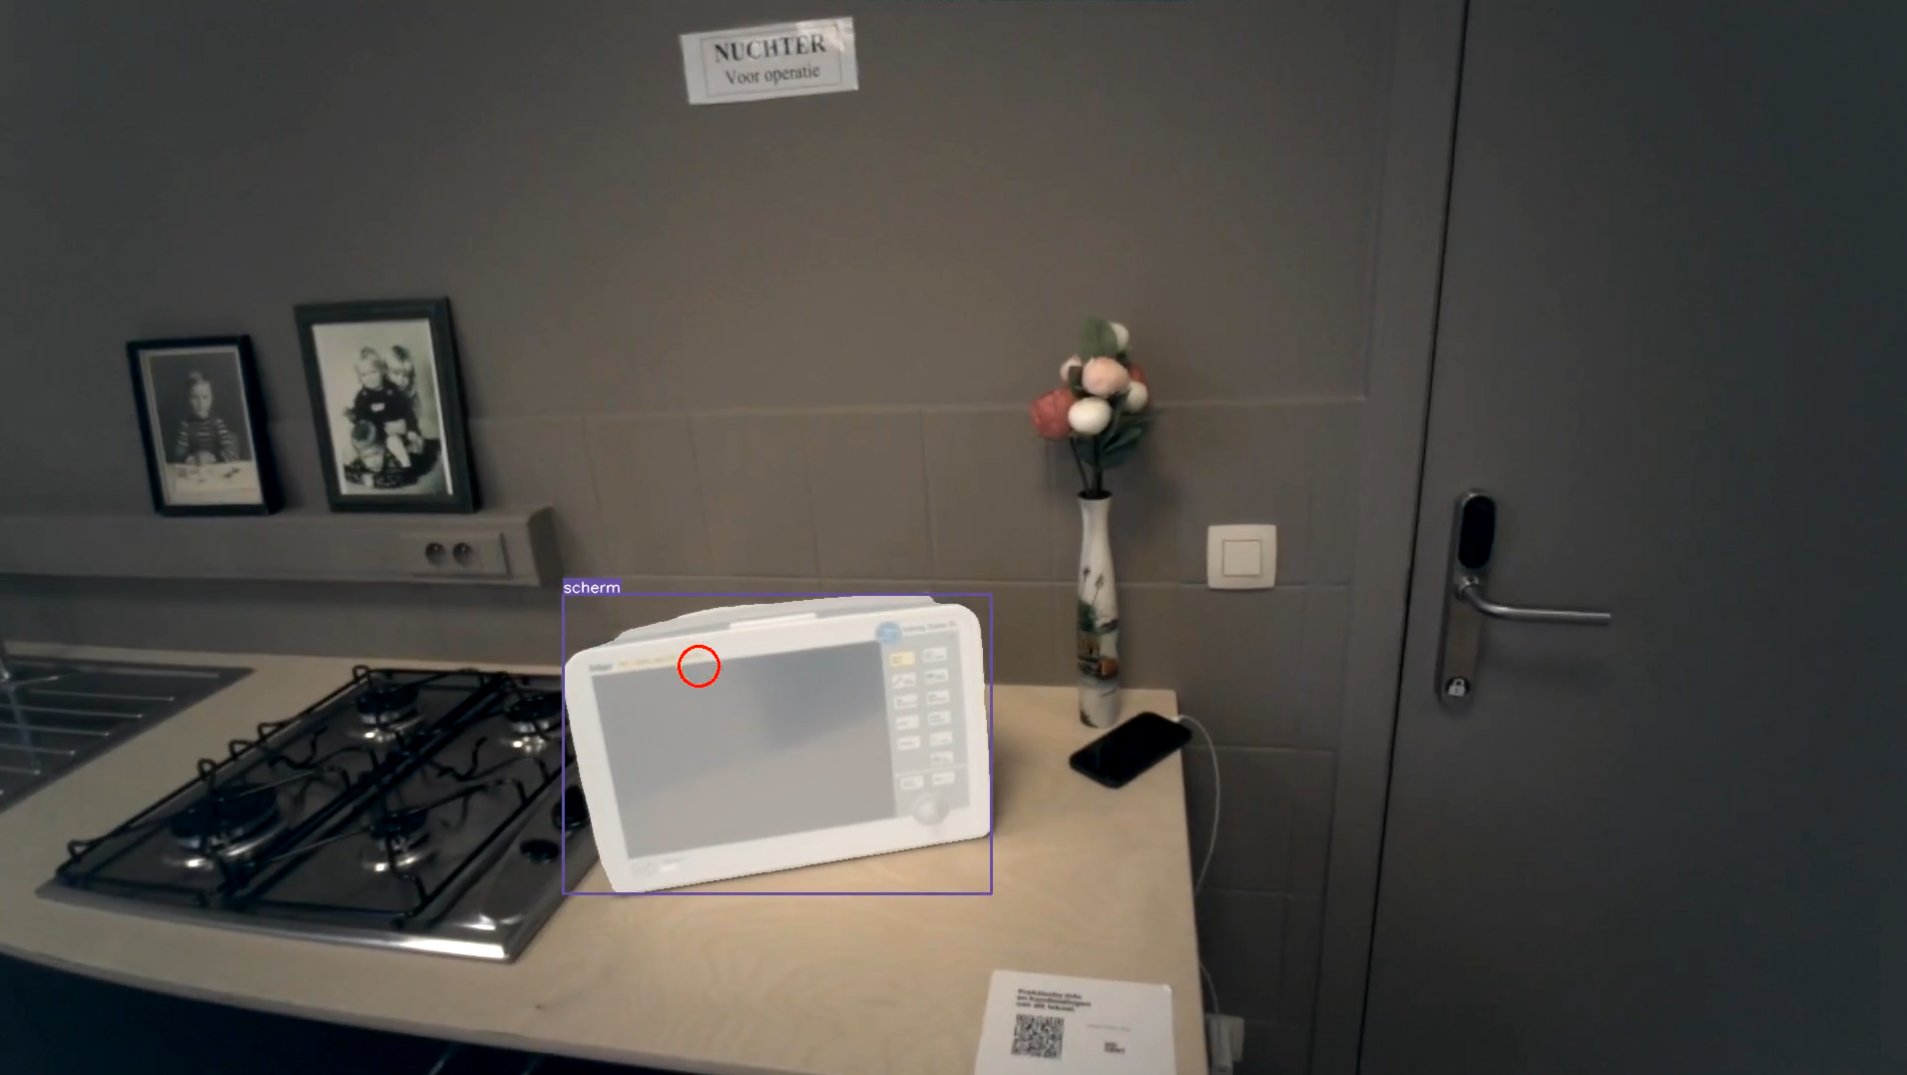
\includegraphics[width=0.8\textwidth]{voorbeeld_labeling_validatie.png}
%   \caption[]{\label{fig:object-detection}Voorbeeld van een frame in een video voor labeling-validatie. Hier kijkt de deelnemer naar een scherm, waarbij het segmentatiemasker, de bounding box, het blikpunt en het objectlabel weergegeven worden.}
% \end{figure}

\section{Analyse van de Experimentele Data}

Tenslotte werd de verzamelde data geanalyseerd met behulp van verschillende computer vision technieken.
De focus lag op het evalueren van de betrouwbaarheid van de analyses, door ze te vergelijken met de handmatig gelabelde grondwaarheid die tijdens het experiment was verzameld.
De resultaten van deze evaluatie worden gepresenteerd in Hoofdstuk~\ref{ch:analyse}.

TODO: dit deel uitbreiden